% !TeX root = report.tex
% !TeX encoding = UTF-8
% !TeX spellcheck = en_US
% !TeX document-id = {b18791db-4bf7-45f4-b2cb-865b91539759}
%
% Report for Student Intervention System
% Udacity MLND Project 2
%
% Aravind Battaje

\documentclass{article}

% Packages used
\usepackage[margin=1in]{geometry}
\usepackage{multirow}
\usepackage{booktabs}
\usepackage{graphicx}
\usepackage{caption}
\usepackage{subcaption}
\usepackage{amsmath}

% Begin document
\begin{document}
	
	\title{Project Report: Student Intervention System}
	\author{Aravind Battaje}
	\maketitle
	
	\section{Project Steps}
	The goal of the project is to find a suitable supervised machine learning algorithm that can identify students who might need early intervention, by predicting their success/failure in graduation from the current records. To accomplish this task, three supervised learning models are probed for their suitability, and the best of them is later fine-tuned to get the best possible learning algorithm. All the three models are realized with the help of \texttt{scikit-learn}. For each of three models, a preliminary analysis is performed about its suitable basic configuration, costs and performance. Because of the small size of the dataset, cost and performance are measured by running multiple trials on shuffled data. The overall best performer that balances cost and performance is then fine-tuned using grid search (on parameters) and final predictions are made.
	
	
	\section{Classification vs Regression}
	A machine learning algorithm can be classified into two types, based on its nature of outputs, viz., classification and regression. Classification supports outputs of discrete values and regression outputs continuous values. This project entails a classification type of problem because the output desired from the \emph{intervention system} is discrete in nature, i.e., a student graduates or not from his/her current characteristics. Regression would be more suitable for, say an algorithm that predicts the final exam score from a student's current academic records.
	
	
	\section{Dataset}
	Several qualities of students such as their family background, social characteristics, extra-curricular activities, etc., along with the information if they graduated or not, are given along with the project in \texttt{student-data.csv}. The dataset possesses following characteristics:
	\begin{center}
		\begin{tabular}{c|c}
			\toprule
			Total number of students & 395 \\
			Number of students who passed & 265 \\
			Number of students who failed & 130  \\
			Graduation rate of the class & 67.09\% \\
			Number of features of dataset & 30 \\
			\bottomrule
		\end{tabular}
		\label{tab:data_characteristics}
	\end{center}
	
	
	\section{Training and Evaluating Models}
	Three supervised learning algorithms from \texttt{scikit-learn} were probed for their potential in \emph{best} modeling the student intervention problem. 
	
	\subsection{Naive Bayes Classifier}
	Naive Bayes Classifier is one of the simplest, and yet powerful algorithms used in supervised learning. It is a subset of the more complex generalization - Bayesian inference - in that, the likelihood of a hypothesis for modeling the data is inferred from the likelihood of data given a hypothesis. A contrived example which uses some of the features of the data provided in this project (\texttt{student-data.csv}) illustrates a few basic principles. Figure \ref{fig:belief_bayesian_inference} shows a belief network modeled with the classification variable \emph{passed} dependent on three features, with a certain conditionality evident between them. From the data (training), conditional probabity tables for each node is calculated, and so when a new data sample (testing) is introduced, the joint probability for \emph{passed} is calculated by simply multiplying relevant entries from the table. That is, assuming $v_1$, $v_2$ and $v_3$ represent the variables from the sample for \emph{goout}, \emph{freetime} and \emph{failures} respectively, 
	\[P(passed=1, goout=v_1, freetime=v_2, failures=v_3)\] will give the probabilty of student passing. This joint probability can be expressed as, \[P(...) = \prod_{i=1}^{n}P(v_i|Parents(Y_i)),\] where $P(passed=1)$, $P(goout=v_1|passed=1)$, $P(freetime=v_2|passed=1)$ and $P(failures=v_3|freetime=v_2,goout=v_1)$ will be the individual terms, derived from the belief network.
	
	\begin{figure}[h]
		\centering
		\begin{subfigure}[h]{0.4\textwidth}
			\centering
			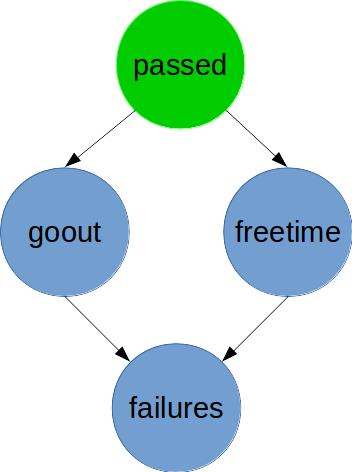
\includegraphics[scale=0.4]{example_belief_network_full}
			\caption{Bayesian Inference}
			\label{fig:belief_bayesian_inference}
		\end{subfigure}
		\begin{subfigure}[h]{0.4\textwidth}
			\centering
			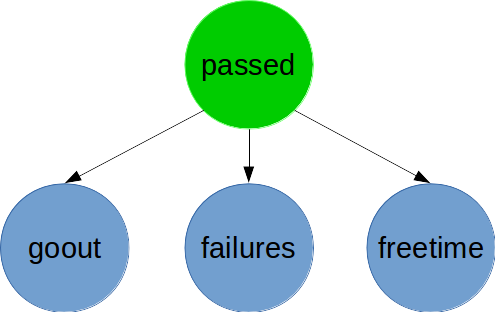
\includegraphics[scale=0.4]{example_belief_network_naive}
			\caption{Naive Bayes}
			\label{fig:belief_naive_bayes}
		\end{subfigure}
		\caption{Example belief networks with some of the features of \texttt{student-data}. \emph{passed} is the classification variable indicating if a student will pass or not; \emph{goout} indicates the time spent by a student going out with friends; \emph{freetime} indicates the free time a student gets after school; and, \emph{failures} indicates a student's failures in the past.}
	\end{figure}
	
	Naive Bayes Classifier shown in Figure \ref{fig:belief_naive_bayes} on the other hand assumes conditional independence between the features, and models the classification variables as being directly dependent on all features. The joint probability $P(passed=1, goout=v_1, freetime=v_2, failures=v_3)$ thus is much simpler: \[P(...) = P(passed=1)P(goout=v_1|passed=1)P(freetime=v_2|passed=1)P(failures=v_3|passed=1)\] 
	Computationally this is cheaper than the more complicated belief network of Figure \ref{fig:belief_bayesian_inference}, but more importantly, the computational cost of finding the best arrangement of nodes in the belief network during training grows exponentially with number of nodes (or features). Therefore, Bayesian inference - ideally considered as the \emph{gold} standard for supervised learning - becomes impractical. 
	
	Nevertheless, Naive Bayes still stands out pretty well even as it assumes no causality between the several features of the data. It has been shown to work surprisingly well in many applications, especially in spam-filtering and such text-based classifiers \cite{Metsis06}. Although the dataset provided along with the project doesn't qualify as having much text based data, and it could sway more towards a dataset which has correlated data features, such as in Figure \ref{fig:belief_bayesian_inference}, it has been shown that even with the independence assumption on dependent features, as in Figure \ref{fig:belief_naive_bayes}, Naive Bayes works pretty well \cite{Rish01}. Naive Bayes classifier is also extrememly computationally efficient for both training and predicting considering the amount of calculations involved and it could ideally set a benchmark for the other algorithms to compete against. However, the downside is that the dataset size is quite small considering the number of features, and so Naive Bayes is susceptible to the \emph{curse of dimensionality}.

	\begin{table}[h]
		\centering
		\begin{tabular}{l|ccc}
			\toprule
			{} & \multicolumn{3}{c}{Training set size} \\
			{} &       100 &       200 &       300 \\
			\midrule
			Training time (msec)                  &  1.136737 &  1.401565 &  1.677573 \\
			Prediction time - Training set (msec) &  0.539596 &  0.743282 &  0.940869 \\
			Prediction time - Testing set (msec)  &  0.535090 &  0.538042 &  0.541995 \\
			F1 score - Training set               &  0.703436 &  0.800078 &  0.797350 \\
			F1 score - Testing set                &  0.613627 &  0.746451 &  0.752224 \\
			\bottomrule
		\end{tabular}
		\caption{Performance of Naive Bayes Classifier (100 runs)}
		\label{tab:naive_bayes_100}
	\end{table}
	
	\texttt{scikit-learn}'s \texttt{GaussianNB()} is used to train 300 samples from the given dataset in default setting; no additional parameters are provided. This process is repeated for 100 runs and the obtained mean performance is logged in Table \ref{tab:naive_bayes_100}. It can be seen that the training times for the classifier is in the order of a millisecond, and it seems to grow linearly with the training set size. The same holds true for prediction times, and the $F_1$ scores on the test data for a training set size of 300 is remarkable, given the computational cost. 
	        
	\subsection{Support Vector Machine}
	Support Vector Machines (SVM) is one of the most ubiquitous supervised learning algorithms in the realm of statistical inference and machine learning. It is exemplary of a class of classifiers that try to maximize the \emph{margin} for a decision boundary between two classes \cite{boser1992}. Data (or model) generalization -- at least to some extent -- is thus inherently a part of SVM, as the maximum margin ensures that the decision boundary is not too close to the data points, which should prevent over-fitting. It is also incredibly economical as computing of maximum margin and the decision boundaries really boils down to dot products of data sample vectors in the former and data sample vector with sample to predict for the latter. In its simplest form, SVM based classifier (SVC) linearly separates data points with the maximum margin hyper-plane. To work on non-linearly separable data, SVM algorithm also makes it very easy to use \emph{kernel trick} in the model; the previously noted dot product advantage makes the application of a kernel on the data have barely any computational overhead. 
	
	Figure \ref{fig:svc_rbf_example} shows a contrived example that considers two non-linearly separable features from the given dataset. It illustrates the extension of the nascent form of SVC (linear separator) with a simple radial basis function (RBF) kernel. It can be seen that the RBF kernel allows formation of complex decision boundaries within the rules of maximum \emph{soft} margin, and fits the data pretty well. 
	
	SVC has been proven to work extremely well for text recognition and categorization tasks \cite{boser1992,joachims1998}, such as in optical character readers. It indicates the nature of SVC to adapt to highly non-linear and inter-dependent data features. In the dataset given, it can be said that some of the features are interdependent to an extent, and more importantly are highly non-linear in nature, with an exaggerated sense of discreteness (2 or 3 values). Additionally, SVMs are very amenable to non-linear score metrics such as $F_1$ score used in the project \cite{joachims2005}. Thus SVC should ideally suit the student intervention system context naturally.
	
	\texttt{scikit-learn} provides \texttt{SVC()} that is capable of working with several types of kernels and parameters. Single runs -- training and testing -- with \texttt{SVC()} having \emph{linear}, \emph{rbf}, \emph{poly} (\emph{degree} 2 and 3), and \emph{sigmoid} kernels were performed. The (rough) performance extracted from the single runs are then used to decide on the \emph{best} kernel configuration for the context. For all the runs, \emph{best practices} for SVMs \cite{hsu2003} were followed, such as scaling input data values ($[-1,+1]$) so that the features carry zero mean and unit variance. Before scaling, the dataset was shuffled and split into 300 data points for training (later used in subsets) and the rest for testing. The same scaling transformation used for training set was used to scale the test set at the time of \texttt{predict}. \emph{linear} kernel was found to be fast, but performed on par with Naive Bayes classifier in terms of $F_1$ score. \emph{poly} (\emph{degree} 3) kernel's performance was inconsistent; over-fitting seemed to be imminent from the $F_1$ score. \emph{sigmoid} kernel did not suit the dataset very well; it never made a consistent decision boundary and was independent of the training set size. Two kernels, viz., \emph{rbf} and \emph{poly} (\emph{degree} 2) were found to perform well on the dataset. 100 trials with shuffled datasets were performed on each of the these kernels and the mean performance was recorded. Table \ref{tab:svc_poly_100} records the performance of \emph{poly} (\emph{degree} 2) kernel, and Table \ref{tab:svc_rbf_100} records that of \emph{rbf} kernel. With 100 runs, similarities in their performance becomes prevalent; $F_1$ scores on the test data set seem to be very close to each other. Objectively \emph{poly} kernel is seems to be better than \emph{rbf} because of the lesser training and prediction times, but given the robustness of \emph{rbf} in other application domains \cite{hsu2003}, it wins out against \emph{poly}.  
	
	\begin{figure}[t]
		\centering
		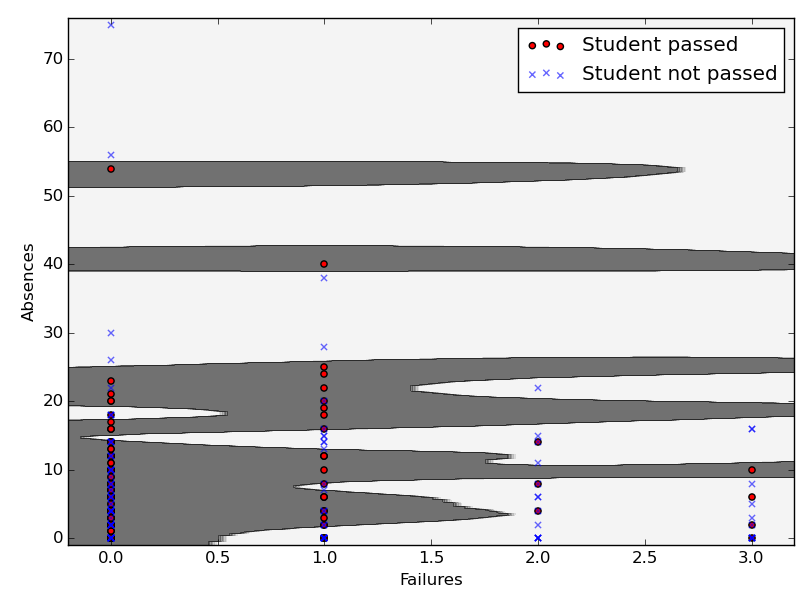
\includegraphics[scale=0.5]{example_svc}
		\caption{Example Support Vector Machine based Classifier with an RBF kernel; \emph{Failures} indicates a student's past failures; \emph{Absences} indicates number of classes a student was absent for. Decision boundaries in grey (student passed) and white (student not passed) are underlying the data points of \emph{passed} label from the dataset.}
		\label{fig:svc_rbf_example}
	\end{figure}
	
	\begin{table}[h]
		\centering
		\begin{tabular}{l|ccc}
			\toprule
			{} & \multicolumn{3}{c}{Training set size} \\
			{} &       100 &       200 &       300 \\
			\midrule
			Training time (msec)                  &  1.436007 &  4.016979 &  8.038867 \\
			Prediction time - Training set (msec) &  0.798676 &  2.626345 &  5.504694 \\
			Prediction time - Testing set (msec)  &  0.758820 &  1.313007 &  1.809123 \\
			F1 score - Training set               &  0.912564 &  0.903239 &  0.895141 \\
			F1 score - Testing set                &  0.794443 &  0.790969 &  0.792418 \\
			\bottomrule
		\end{tabular}
		\caption{Performance of SVC Polynomial $2^{nd}$ degree Kernel (100 runs)}
		\label{tab:svc_poly_100}
	\end{table}
	
	\begin{table}[!ht]
		\centering
		\begin{tabular}{l|ccc}
			\toprule
			{} & \multicolumn{3}{c}{Training set size} \\
			{} &       100 &       200 &       300 \\
			\midrule
			Training time (msec)                  &  1.720572 &  5.235305 &  10.758593 \\
			Prediction time - Training set (msec) &  1.102505 &  3.869443 &   8.228962 \\
			Prediction time - Testing set (msec)  &  1.050613 &  1.893101 &   2.676311 \\
			F1 score - Training set               &  0.927031 &  0.911822 &   0.904793 \\
			F1 score - Testing set                &  0.800927 &  0.805108 &   0.808884 \\
			\bottomrule
		\end{tabular}
		\caption{Performance of SVC RBF Kernel (100 runs)}
		\label{tab:svc_rbf_100}
	\end{table}
	
	\subsection{Boosting}
	
	Boosting is a class of ensemble-based supervised learning (meta-)algorithms that follow the principle of assembling a \emph{strong} estimator from a bunch of \emph{weak} estimators. By definition, a \emph{weak} estimator has a performance only better than predicting by chance, i.e., error of lesser than 0.5 in binary classification. Boosting iteratively tries to fit these \emph{weak} estimators to the data by exaggerating weights of the samples that were misclassified in the previous iteration. This effectively changes the \emph{distribution} of data samples from the perspective of the \emph{weak} learners or hypotheses. The final hypothesis then will be similar to a weighted sum of the individual hypotheses gathered in each iteration. The weights are a function of the prediction error in the iteration. This simple technique of adapting weak estimators to form a voting (vaguely) ensemble is very powerful \cite{shapire1990}, and a robust, well-proven version of it, called \emph{AdaBoost} \cite{Freund1997} is used here. Quite surprisingly, it has been shown that AdaBoost (and boosting in general) is highly resistant to overfitting \cite{Schapire2013}, given truly \emph{weak} estimators are used, sufficient margins are created in each iteration and data is not too noisy. Thus, Boosting could ideally be the best algorithm for this project. The downside however, could be the (linearly) scaling computational cost, which gets added up from the individual estimators.
	
	\begin{table}[h]
		\centering
		\begin{tabular}{l|ccc}
			\toprule
			{} & \multicolumn{3}{c}{Training set size} \\
			{} &         100 &         150 &         200 \\
			\midrule
			Training time (msec)                  &  116.995811 &  116.348028 &  116.556168 \\
			Prediction time - Training set (msec) &    8.880124 &    9.707942 &   10.348394 \\
			Prediction time - Testing set (msec)  &    8.139987 &    8.327084 &    8.233488 \\
			F1 score - Training set               &    0.951172 &    0.864298 &    0.819485 \\
			F1 score - Testing set                &    0.586345 &    0.614715 &    0.622481 \\
			\bottomrule
		\end{tabular}
		\caption{Performance of AdaBoost Classifier (100 runs)}
		\label{tab:adaboost_weak_100}
	\end{table}
	
	\texttt{AdaBoostClassifier()} from \texttt{scikit-learn} makes it possible to run any \emph{weak} base estimator that supports sample weighting. In the project, \texttt{DecisionTreeClassifier()} is used as base estimator. Since decision trees have a natural tendency to bias towards the dominant class label, and the dataset provided along with the project has more \texttt{'passed == 'yes'} labels,  \emph{data balancing} was performed. This step entails eliminating entries in the dataset that pertain to the dominant label, to equalize with number of non-dominant ones. The number of samples was thus reduced to 260 from the 365 of the unbalanced dataset. So the shuffle-split procedure results in 200 training and 60 test samples, and the training set sizes becomes 100, 150 and 200. Table \ref{tab:adaboost_weak_100} shows this difference in training set sizes, in comparision to previous algorithms such as in Table \ref{tab:naive_bayes_100}. 
	
	With the above mentioned data balancing setup, sample runs with two configurations are performed. First, a strong base estimator, i.e., a decision tree of \texttt{max\_depth} 15 is used. It was observed that training $F_1$ scores were always $1.0$ for all training sizes. This shows the potential of overfitting with AdaBoost due to non-adherence of the weak estimator clause. The second (practical configuration) uses a weak decision tree (stump) with \texttt{max\_depth} 1 as its base estimator. A sample run with this configuration is verified to be better than first, and so performance is measured by averaging 100 runs. This is shown in Table \ref{tab:adaboost_weak_100}. It is apparent from the table that the training times is almost an order of magnitude more than the previous models, but it remains more or less constant with different training set sizes because AdaBoost stops at a specified number of iterations (\texttt{n\_estimators}), and doesn't directly depend on the input size. More importantly, although the $F_1$ scores seem to be much lesser than the previous models on test set, it is only as a consequence of \emph{data balancing}. So given the different dataset sizes, there is no direct way to compare between models directly, but it can be seen later that AdaBoost's performance is really not as low as it seems. Section \ref{general_issues} has more details about this \emph{issue}. In any case, it can be concluded that with the given dataset, AdaBoost doesn't perform very well, or the $F_1$ scores are on par with Naive Bayes model. This could change however with a larger, and preferably already balanced, dataset.
	
	\section{General Issues} \label{general_issues}
	
	\section{Finding the Best Model}
	Out of the three models tried above, Support Vector Machine based classifier that uses a radial basis function kernel stands unbeaten. 
	
	\section{Notes}
	Use of Neural Networks was considered, but scikit-learn (stable) doesn't directly support multi-layer perceptron currently. Although other libraries (Theano, scikit-neuralnetwork) could be used, exploration has been pushed forward both because it was suggested to "choose 3 supervised learning models that are available in scikit-learn", and neural networks will be later encountered during \emph{Deep Learning}.
	
	\bibliography{report}
	\bibliographystyle{alpha}
\end{document}